\documentclass[letterpaper]{article}
\usepackage[margin=.64in]{geometry}
\usepackage{amsmath}
\usepackage{graphicx}

\title{Goldschmidt Integer Divider User Guide}
\date{2021-09-01}
\author{Jose R. Garcia}

\begin{document}
	\pagenumbering{gobble}
	\maketitle
	\newpage
	\pagenumbering{arabic}
	
	\tableofcontents
    \newpage
    
	\section{Abstract}
	
	The Goldschmidt integer divider written in verilog. Similar to Newton-Raphson but the division step can be pipelined. This document contains and overview of the design and guidance on the usage and integration of this component.
	
	\section{Syntax and Abbreviations}
	
	\begin{tabular}{l|l}
		Term & Definition \\
		\hline
		0b0 & Binary number syntax \\
		\hline
		0x0000\_0000 & Hexadecimal number syntax \\
		\hline
		bit & Single binary digit (0 or 1) \\
		\hline
		BYTE & 8-bits wide data unit \\
		\hline
		DWORD & 32-bits wide data unit \\
		\hline
		FPGA & Field Programmable Gate Array \\
		\hline
		GCD & Goldschmidt Convergence Division \\
		\hline
		LSB & Least Significant bit \\
		\hline
		MSB & Most Significant bit \\
		\hline
		WB & Wishbone Interface \\
	\end{tabular}
	
	\section{Design}
	\paragraph{}
	The Goldschmidt division is an special application of the Newton-Raphson method. This iterative divider computes:
	\begin{equation*}
	d(i) = d[i-1].(2-d[i-1])
	\end{equation*}
	\begin{equation*}
	D(i) = D[i-1].(2-d[i-1])
	\end{equation*}
	were \( d \) is the divisor; \( D \) is the dividend; \( i \) is the step. \( D \) converges toward the quotient and d converges toward 1 at a quadratic rate. For the divisor to converge to 1 it must obviously be less than 2 therefore integers greater than 2 must be multiplied by 10 to the negative powers to shift the decimal point. Consider the following example: $ \dfrac{16}{4} $
	
	\begin{tabular}{l|l|l|l}
		Step & D & d & 2-d \\ \hline
		inputs & 16 & 4 & - \\
		0 & 1.6 & 0.4 & 1.6 \\
		1 & 2.56 & 0.64 & 1.36 \\
		2 & 3.4816 & 0.8704 & 1.1296 \\
		3 & 3.93281536 & 0.98320384 & 1.01679616 \\
		4 & 3.99887155603702 & 0.999717889009254 & 1.00028211099075 \\
		5 & 3.99999968165356 & 0.999999920413389 & 1.00000007958661 \\
		6 & 3.99999999999997 & 0.999999999999994 & 1.00000000000001 \\
		7 & 4 & 1 & 1 \\
	\end{tabular}
	
	\paragraph{}The code implementation compares the size of the divisor against $ 2*10^n $ were $ n $ is a natural number. The result of the comparison indicates against which $ 10^m $, were $ m $ is a negative integer, to multiply the divisor. Then the Goldschmidt division is performed until the divisor converges to degree indicated by \textbf{P\_GCD\_ACCURACY}. The quotient returned is the rounded up value to which the dividend converged to. Each Goldschmidt step is performed in to two half steps in order use only half the multipliers and save resources.
	
	The remainder calculation requires an extra clock which is why the address tag is used to make the decision on whether to do the calculation or skip it. The calculation simply takes the value after the decimal point of the quotient a multiplies it by the divisor.
	
	\section{Configurable Parameters}
	
	These are the over-writable parameters.
	
	\begin{tabular}{l|c|l}
		Parameters & Default State & Description \\ \hline
		P\_GID\_FACTORS\_MSB &  31 & Dividend, divisor and results most significant bit. \\ \hline
		P\_GID\_ACCURACY\_LVL & 12 & Divisor Convergence Threshold. How close to one does it get to\\   & & accept the result. These are the 32bits after the decimal point,\\
		& & 0.XXXXXXXX expressed as an integer. The default value represent\\
		& & the 999 part of a 64bit binary fractional number equal to 0.999. \\ \hline
		P\_GID\_ROUND\_UP\_LVL &  2 & Number of bits to look at after the decimal point to round up. \\ 
	\end{tabular}
	
	\section{Clocks and Resets}
	
	This module only possess one clock domain and a synchronous reset signal.
	
    \begin{tabular}{l|c|c|l}
        Signals & Initial State & Direction & Definition \\ \hline
		i\_clk &  N/A & In & Input clock. All interfaces are sampled \\
		       &      &    & on the positive edge of this clock signal. \\  \hline
		i\_reset\_sync & N/A & In & Synchronous reset. Used to reset this unit. \\
	\end{tabular}
	
	\section{Interfaces}
	The divider and divisor are received through i\_master\_div0\_read\_data and i\_master \_div1\_read\_data and qualified by the i\_slave\_stb. The i\_slave\_stb signal could be managed in different ways. It can be a pulse with the width of a singe clock to operate as a pipelined Wishbone interface and the o\_master\_div\_write\_stb can be considered as a Wishbone o\_ack. I can also be operated as a Wishbone standard using those same signals.
	
	When the division concludes  the o\_master\_div\_write\_stb is asserted and writes the result to the address received through i\_slave\_addr.
	\subsection{WB4 Slave}
		
	\begin{tabular}{l|c|c|c|l}
		Signals & Initial State & Dimension & Direction & Definition \\ \hline
		i\_wb4\_slave\_stb &  N/A & 1-bit &  Input & Valid data strobe and start\\
		& & & & indicator. \\  \hline
		i\_wb4\_slave\_data & N/A & [(P\_GID\_FACTORS\_MSB*2)+1:0] & Input & Divisor and Dividend. \\  \hline
		i\_wb4\_slave\_tgd & N/A & [1:0] & Input & Indicates the calculation to\\
		& & & & perform.\\
		& & & & bit[1] 0=quotient, 1=remainder;\\
		& & & & bit[0] 0=signed, 1=unsigned \\  \hline
		o\_wb4\_slave\_stall & N/A & 1-bit & Output & Stall, not ready when set to 1. \\
	\end{tabular}

	\subsection{WB4 Master}
	
	\begin{tabular}{l|c|c|c|l}
		Signals & Initial State & Dimension & Direction & Definition \\ \hline
		o\_wb4\_master\_stb &  N/A & 1-bit &  Input & Valid data strobe and start indicator.\\  \hline
		o\_wb4\_master\_data & N/A & [P\_GID\_FACTORS\_MSB:0] & Output & Operation result.\\  \hline
		i\_wb4\_master\_stall & N/A & 1-bit & Input & Stall, not ready when set to 1. \\
	\end{tabular}
	
	\section{Test Bench and Simulation}
	Test Bench and Simulation
	
	\subsection{Test Bench}
	
	The test bench is written in uvm-python (UVM), it requires cocotb. A Wishbone Slave verification agent stimulates the DUT by sending factors for the DUT to provide the division result. A Wishbone Master verification agent is used as a monitor to capture the result. A predictor sees the Wishbone Slave transactions and consequently generates Wishbone Master transactions to compare against the response generated by the DUT. Figure 1 provides a low detailed description of the test bench components and connections
	
	\begin{figure}[h]
		\centering
		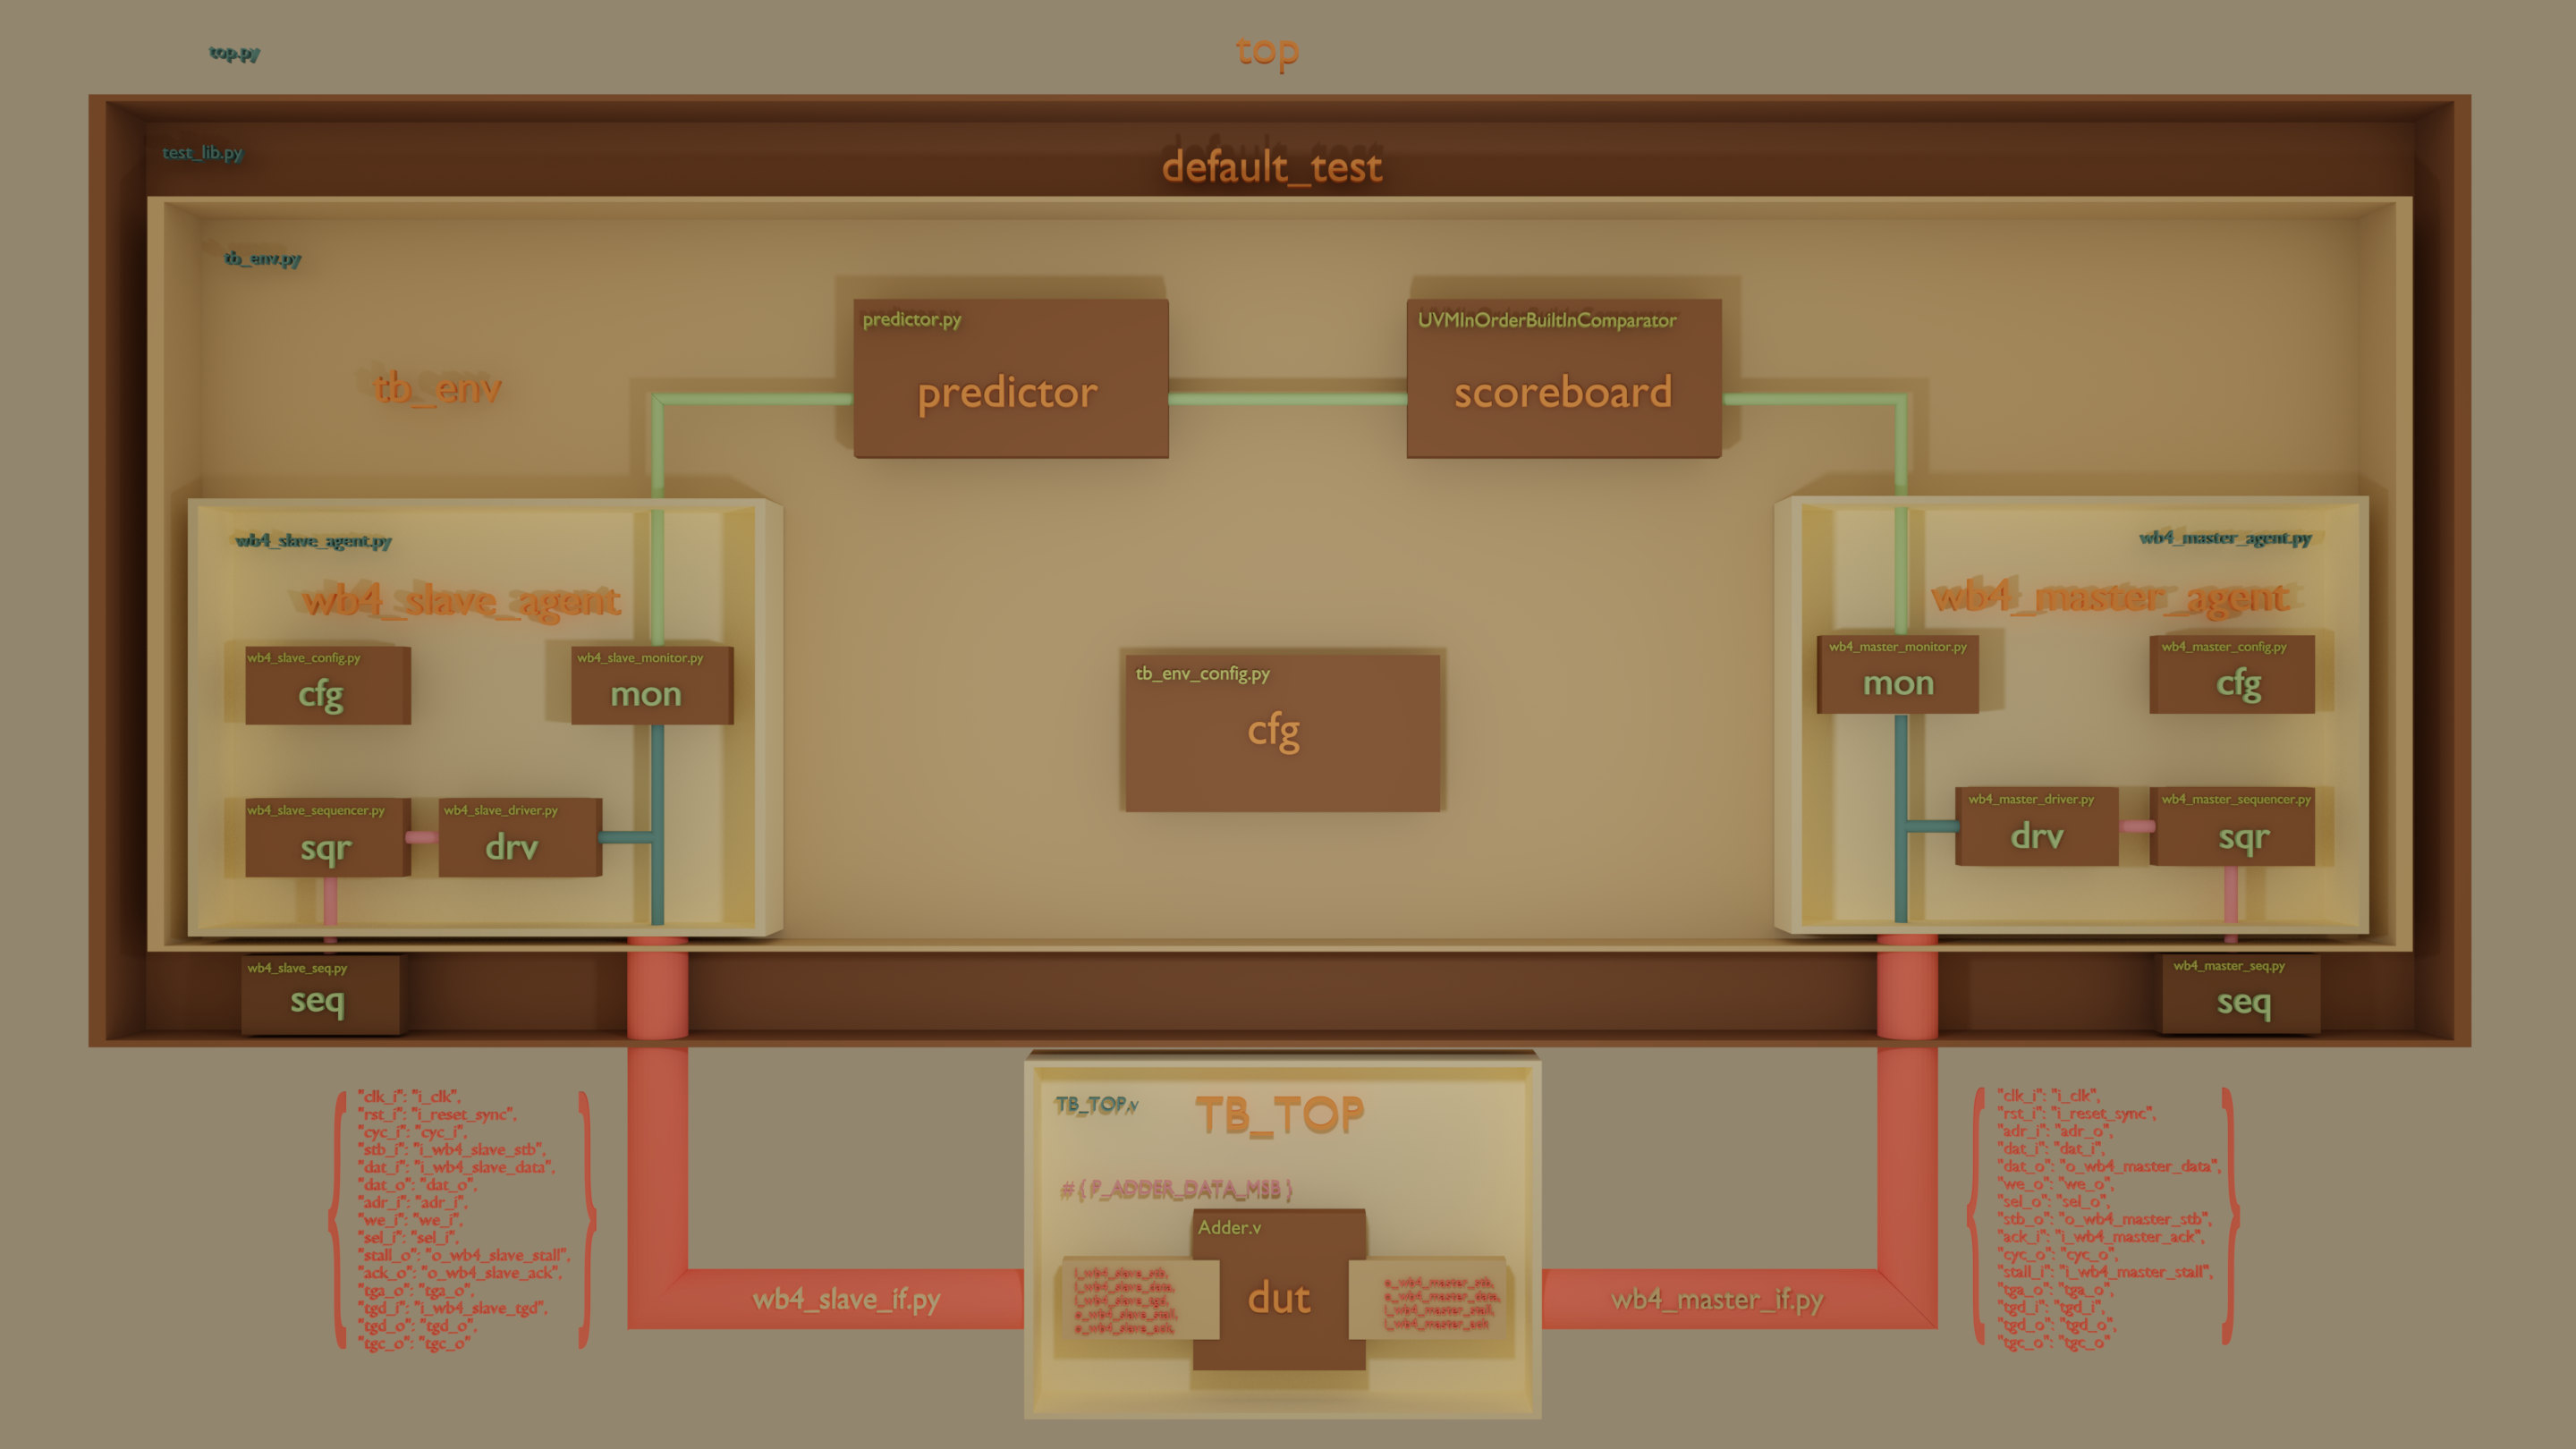
\includegraphics[width=0.99\linewidth]{../figures/tb_diagram}
		\caption[Test Bench Block Diagram]{Test Bench Block Diagram}
		\label{fig:tbdiagram}
	\end{figure}
	
	\subsection{Simulation}
	
	\subsubsection{Prerequisites}
	
	
	\begin{tabular}{l}
	    Verilator(version 4.106) \\
	    cocotb \\
	    cocotb-coverage \\
	    uvm-python \\
	    gtkwave(optional)\\
    \end{tabular}
	
	\paragraph{}To install a simulator follow the instructions in in the verilator website.
	For setting cocotb and uvm-python: 
	
	\begin{tabular}{l}
	    {\tt sudo apt install python3-pip } \\
	    {\tt pip install cocotb } \\
	    {\tt pip install cocotb-coverage } \\
	    {\tt git clone https://github.com/tpoikela/uvm-python.git } \\
	    {\tt cd uvm-python } \\
	    {\tt python -m pip install --user . } \\
    \end{tabular}
	
	
	\subsubsection{Execution}
	
	From the {\tt /Goldschmidt\_Integer\_Divider/sim/ } directory run the command
	
	{\tt make}\\
	
	By default the two clocks per step implementation is used for the simulation. To view the wave form open the file \textbf{wave2.gtkw} with \textbf{gtkwave}. If the one clock per step is selected for simulation use \textbf{wave1.gtkw} for the proper set of signals to be loaded into the wave viewer.
	
	\begin{figure}[h]
		\centering
		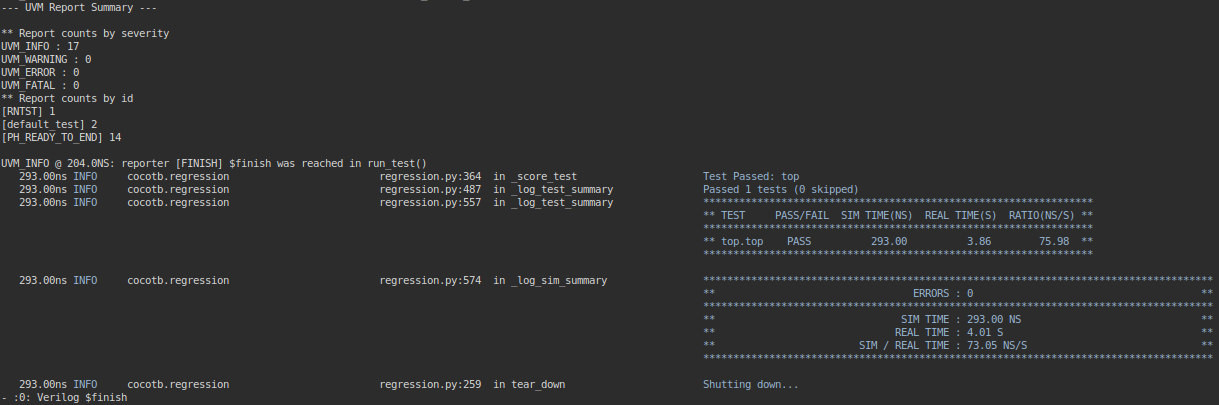
\includegraphics[width=0.99\linewidth]{../figures/Screenshot_sim}
		\caption[sim]{Sim successfully completed.}
		\label{fig:screenshotsim}
	\end{figure}
	
	
\end{document}
